\documentclass{article}

\usepackage{mystyle}

\begin{document}
\section{Notation}
\begin{definition}
Let $d$ be a positive integer. A \emph{partition} of $d$ is an unordered multiset of positive integers $[x_1,\ldots,x_n]$ such that $x_1+\ldots+x_n=d$.
\end{definition}
\begin{definition}
A \emph{combinatorial datum} is a tuple
\[
\mathcal{D}=\datum{\widetilde{\Sigma},\Sigma,d}{\pi_1,\ldots,\pi_n},
\]
where $\Sigma$, $\widetilde\Sigma$ are closed surfaces, $d$ is a positive integer and $\pi_1,\ldots,\pi_n$ are partitions of $d$. The datum $\mathcal{D}$ is \emph{proper} if none of the partitions $\pi_1,\ldots,\pi_n$ is equal to $[1,\ldots,1]$, \emph{improper} otherwise.
\end{definition}

A few remarks about combinatorial data.
\begin{itemize}
\item A combinatorial datum is only defined up to permutation of its partitions. In other words, if two data have the same partitions but in a different order, they are considered equal.
\item When $\Sigma$ is the $2$-sphere, we will often shorten the notation for a combinatorial datum by omitting it:
\[
\mathcal{D}=\datum{\widetilde\Sigma,d}{\pi_1,\ldots,\pi_n}.
\]
\end{itemize}

\begin{definition}
A combinatorial datum
\[
\mathcal{D}=\datum{\widetilde\Sigma,\Sigma,d}{\pi_1,\ldots,\pi_n}
\]
is a \emph{candidate datum} if it satisfies the \emph{Riemann-Hurwitz condition}
\[
\chi(\widetilde\Sigma)-\left(\card{\pi_1}+\ldots+\card{\pi_n}\right)=d\cdot(\chi(\Sigma)-n).
\]
\end{definition}

Let $\Sigma_g$ denote the closed orientable surface of genus $g$. From now on, we will almost always deal with combinatorial data of the form
\[
\datum{\Sigma_g,d}{\pi_1,\pi_2,[s,d-s]}.
\]
In this setting, the Riemann-Hurwitz condition becomes
\begin{equation}\label{eq:rh-n3}
\card{\pi_1}+\card{\pi_2}=d-2g.
\end{equation}

\begin{definition}
A candidate datum $\mathcal{D}$ is \emph{realizable} if it is the combinatorial datum of a branched covering, and is \emph{exceptional} otherwise.
\end{definition}

\section{Combinatorial moves}

\begin{definition}
A \emph{combinatorial move} is a pair of candidate data $\mathcal{D}$, $\mathcal{D}'$ such that $\mathcal{D}$ is realizable provided that $\mathcal{D}'$ is realizable. We use the notation $\mathcal{D}\cmove\mathcal{D}'$ to denote the existence of a combinatorial move between $\mathcal{D}$ and $\mathcal{D}'$.
\end{definition}

This section is devoted to listing several combinatorial moves, which will be used in the next section to classify the realizable candidate data of the form
\[
\datum{\Sigma_g,d}{\pi_1,\pi_2,[s,d-s]}.
\]
We will make extensive use of the following.

\begin{fact*}
A candidate datum $\mathcal{D}=\datum{\Sigma_g,d}{\pi_1,\pi_2,\pi_3}$ is realizable if and only if it admits a \dessin{}, i.e. a graph $\Gamma$ embedded in $\Sigma_g$ with the following properties.
\begin{enumerate}
\item The vertices of $\Gamma$ are colored with two colors, say black and white; each edge of $\Gamma$ has endpoints of different colors.
\item There are $\card{\pi_1}$ black vertices and $\card{\pi_2}$ white vertices in $\Gamma$; $\pi_1$ is the multiset of the degrees of black vertices; similarly, $\pi_2$ is the multiset of the degrees of white vertices.
\item The complement $\Sigma_g\setminus\Gamma$ is the disjoint union of $\card{\pi_3}$ open disks; $\pi_3$ is the multiset of the combinatorial perimeters\footnote{The \emph{combinatorial perimeter} of a disk $D$ in the complement $\Sigma_g\setminus\Gamma$ is the number of edges of $\Gamma$ that make up the perimeter of $D$; edges that do not lie on the boundary of any disk other than $D$ are counted twice.} of these disks divided by $2$.
\end{enumerate}
\end{fact*}

Before we start describing the combinatorial moves, let us introduce a procedure that we will exploit several times in this section. Consider an uncolored graph $\Gamma$ embedded in a surface $\Sigma$, and fix an edge $e$ with endpoints $x$, $y$. The operation of \emph{joining} $x$ and $y$ along $e$ consists in shrinking $e$ to a single point; $x$ and $y$ are merged into a single vertex $z$, whose degree is $\deg{z}=\deg{x}+\deg{y}-2$.

\begin{center}
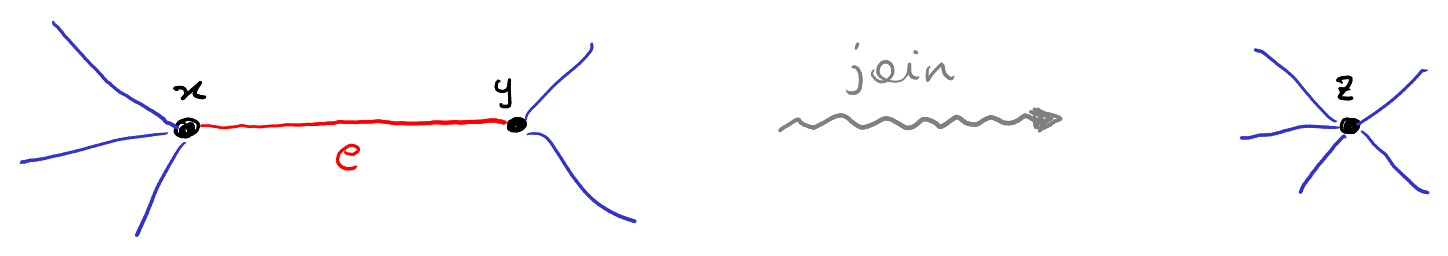
\includegraphics[width=.75\textwidth]{join}
\end{center}

Joining $x$ and $y$ leaves the complement $\Sigma\setminus\Gamma$ topologically unchanged. From a combinatorial point of view, if $\Sigma\setminus\Gamma$ was a disjoint union of open disks, then the same holds after joining; the combinatorial perimeter of the two regions touching $e$ decreases by 1 (if the two regions are the same, then it decreases by 2), while the perimeter of the other regions does not change.

We are now ready to introduce some combinatorial moves. Given a candidate datum $\mathcal{D}=\datum{\Sigma_g,d}{\pi_1,\pi_2,[s,d-s]}$ and a \dessin{} for $\mathcal{D}$, we will conventionally use the color black for the vertices assigned to the partition $\pi_1$, and the color white for the other vertices; each vertex will be labeled with its degree. Moreover, the disk with perimeter $2s$ will be colored orange, and the disk with perimeter $2(d-s)$ will be colored pink.

\begin{combinatorialmove}\label{move:s1-3}
Let $\mathcal{D}=\datum{\Sigma_g,d}{\pi_1,\pi_2,[1,d-1]}$ be a proper candidate datum. Assume that:
\begin{enumerate}
\item $g\ge 1$;
\item there is an element $x\in\pi_1$ such that $x\ge 3$.
\end{enumerate}
Let $x_1$, $x_2$, $x_3$ be positive integers whose sum equals $x$, and consider the partitions
\begin{align*}
\pi_1'=\pi_1\setminus[x]\cup[x_1,x_2,x_3],&&\pi_2'=\pi_2.
\end{align*}
Then
\[
\mathcal{D'}=\datum{\Sigma_{g-1},d}{\pi_1',\pi_2',[1,d-1]}
\]
is a proper candidate datum and $\mathcal{D}\cmove\mathcal{D}'$.
\end{combinatorialmove}
\begin{proof}
Consider a \dessin{} $\Gamma'$ realizing $\mathcal{D}'$. Since the orange disk has perimeter $2$, every vertex of $\Gamma'$ must touch the pink disk. We perform the following operations.
\begin{enumerate}
\item Attach a tube to $\Sigma_{g-1}$ with both endpoints in the pink disk (effectively increasing the genus by $1$).
\item Connect the black vertices of $\Gamma'$ labeled $x_1$, $x_2$, $x_3$ to a dummy black vertex $v$ as shown in the picture.
\item Join $x_1$, $x_2$, $x_3$ and $v$ along the red edges.
\end{enumerate}
\begin{center}
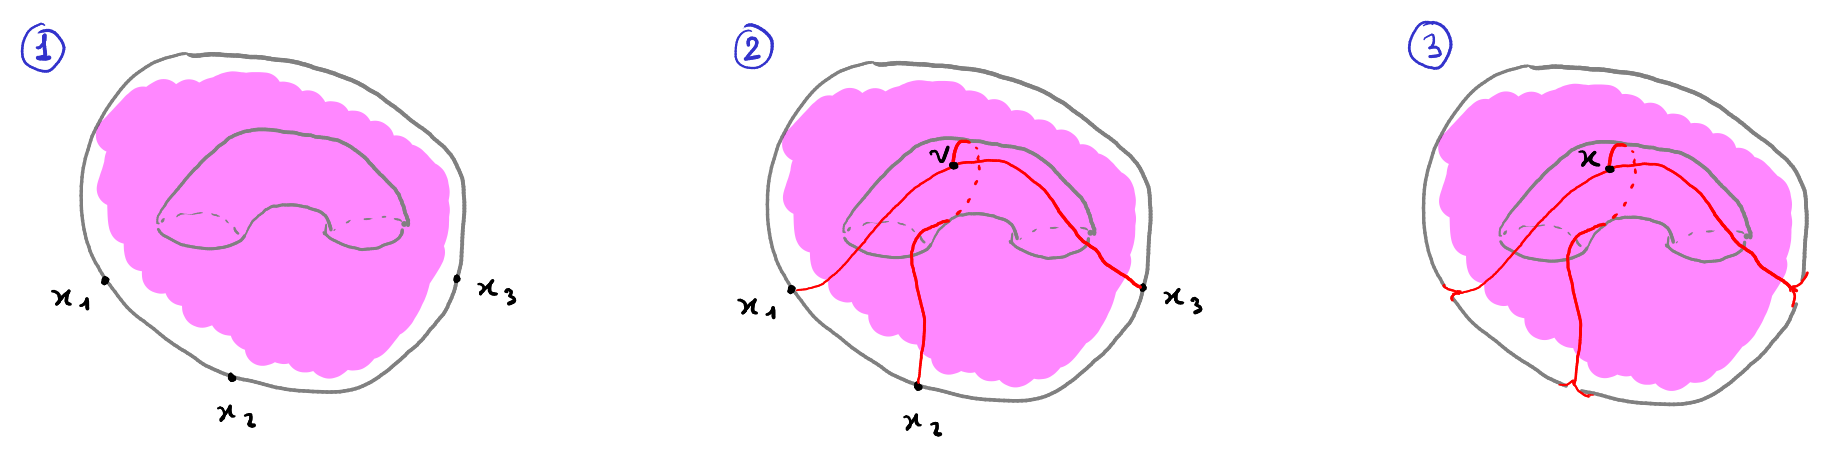
\includegraphics[width=.9\textwidth]{move1}
\end{center}
After these operations, we get a new \dessin{} $\Gamma$. It's easy to check that $\Gamma$ realizes the candidate datum $\mathcal{D}$.
\end{proof}

\begin{combinatorialmove}\label{move:s2-23-22}
Let $\mathcal{D}=\datum{\Sigma_g,d}{\pi_1,\pi_2,[2,d-2]}$ be a proper candidate datum. Assume that:
\begin{enumerate}
\item $[x,y]\subs\pi_1$ for some $x\ge 2$, $y\ge 3$;
\item $[2,2]\subs\pi_2$.
\end{enumerate}
Consider the partitions
\begin{align*}
\pi_1'=\pi_1\setminus[x,y]\cup[x+y-4],&&\pi_2'=\pi_2\setminus[2,2].
\end{align*}
Then
\[
\mathcal{D'}=\datum{\Sigma_g,d-4}{\pi_1',\pi_2',[d-4]}
\]
is a proper candidate datum and $\mathcal{D}\cmove\mathcal{D}'$. In particular, $\mathcal{D}$ is always realizable.
\end{combinatorialmove}
\begin{proof}
Consider a \dessin{} $\Gamma'$ realizing $\mathcal{D}'$. We perform the following operations.
\begin{enumerate}
\item Take the black vertex of $\Gamma'$ labeled $x+y-4$ and split it into two vertices with degrees $x-2$ and $y-2$.
\item Add two white vertices as shown in the picture.
\end{enumerate}
\begin{center}
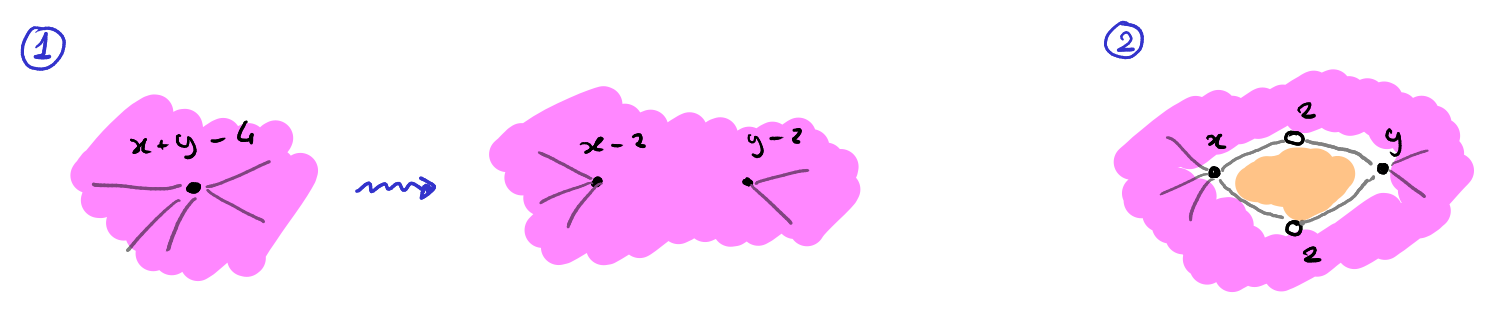
\includegraphics[width=.9\textwidth]{move2}
\end{center}
After these operations, we get a new \dessin{} $\Gamma$. It's easy to check that $\Gamma$ realizes the candidate datum $\mathcal{D}$.
\end{proof}

\begin{combinatorialmove}\label{move:113}
Let $\mathcal{D}=\datum{\Sigma_g,d}{\pi_1,\pi_2,[s,d-s]}$ be a proper candidate datum. Assume that:
\begin{enumerate}
\item $g\ge 1$;
\item $[1,1,3]\subs\pi_1$.
\end{enumerate}
Consider the partitions
\begin{align*}
\pi_1'=\pi_1\setminus[3]\cup[1,1,1],&&\pi_2'=\pi_2.
\end{align*}
Then
\[
\mathcal{D'}=\datum{\Sigma_{g-1},d}{\pi_1',\pi_2',[s,d-s]}
\]
is a proper candidate datum and $\mathcal{D}\cmove\mathcal{D}'$.
\end{combinatorialmove}
\begin{proof}
Consider a \dessin{} $\Gamma'$ realizing $\mathcal{D}'$. Since $[1,1,1,1,1]\subs\pi_1'$, we can assume without loss of generality that there are at least three black vertices labeled $1$ touching the pink disk. Then we can follow the strategy presented in the proof of \cref{move:s1-3} (with $x_1=x_2=x_3=1$) to obtain a new \dessin{} $\Gamma$ which realizes the candidate datum $\mathcal{D}$.
\end{proof}

\begin{combinatorialmove}\label{move:4-2}
Let $\mathcal{D}=\datum{\Sigma_g,d}{\pi_1,\pi_2,[s,d-s]}$ be a proper candidate datum. Assume that:
\begin{enumerate}
\item $2\le s\le d-2$;
\item $g\ge 1$;
\item there is an element $x\in\pi_1$ such that $x\ge 4$;
\item $2\in\pi_2$.
\end{enumerate}
Let $x_1$, $x_2$ be positive integers whose sum equals $x-2$, and consider the partitions
\begin{align*}
\pi_1'=\pi_1\setminus[x]\cup[x_1,x_2],&&\pi_2'=\pi_2\setminus[2].
\end{align*}
Then
\[
\mathcal{D'}=\datum{\Sigma_{g-1},d-2}{\pi_1',\pi_2',[s-1,d-s-1]}
\]
is a proper candidate datum and $\mathcal{D}\cmove\mathcal{D}'$.
\end{combinatorialmove}
\begin{proof}
Consider a \dessin{} $\Gamma'$ realizing $\mathcal{D}'$. There are two cases.
\begin{manycases}[Case \arabic*:]

\case the vertex labeled $x_1$ touches the orange disk and the vertex labeled $x_2$ touches the pink disk (or vice versa). Then we perform the following operations.
\begin{enumerate}
\item Attach a tube to $\Sigma_{g-1}$ with one endpoint in the orange disk and the other in the pink one.
\item Add one black vertex and one white vertex as shown in the picture.
\item Perform the joining operation along the red edges, replacing the black vertices labeled $x_1$, $x_2$ and $2$ with a vertex of degree $x$.
\end{enumerate}
\begin{center}
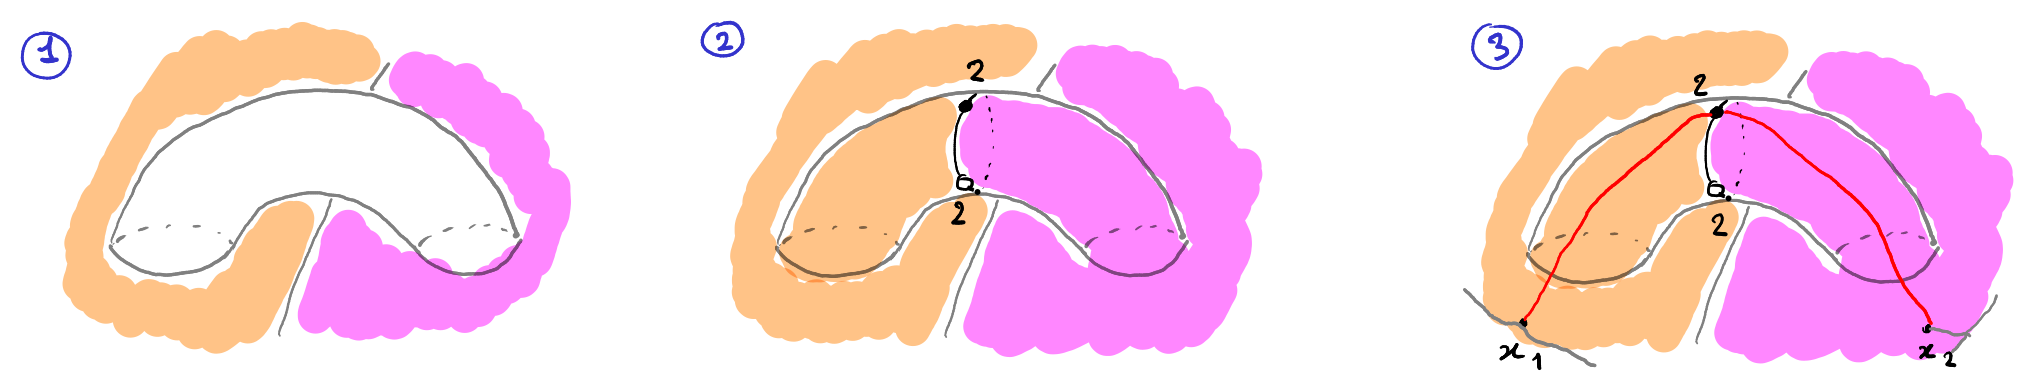
\includegraphics[width=.9\textwidth]{move4-1}
\end{center}
After these operations, we get a new \dessin{} $\Gamma$. It's easy to check that $\Gamma$ realizes the candidate datum $\mathcal{D}$.
\case both the vertices labeled $x_1$ and $x_2$ touch (say) the pink disk. Fix an edge $e$ of $\Gamma'$ that lies on the boundary of both disks. We perform the following operations.
\begin{enumerate}
\item Add one black vertex and one white vertex on $e$ as shown in the picture.
\item Attach a tube to $\Sigma_{g-1}$ with both endpoints in the pink disk.
\item Perform the joining operation along the red edges, replacing the black vertices labeled $x_1$, $x_2$ and $2$ with a vertex of degree $x$.
\end{enumerate}
\begin{center}
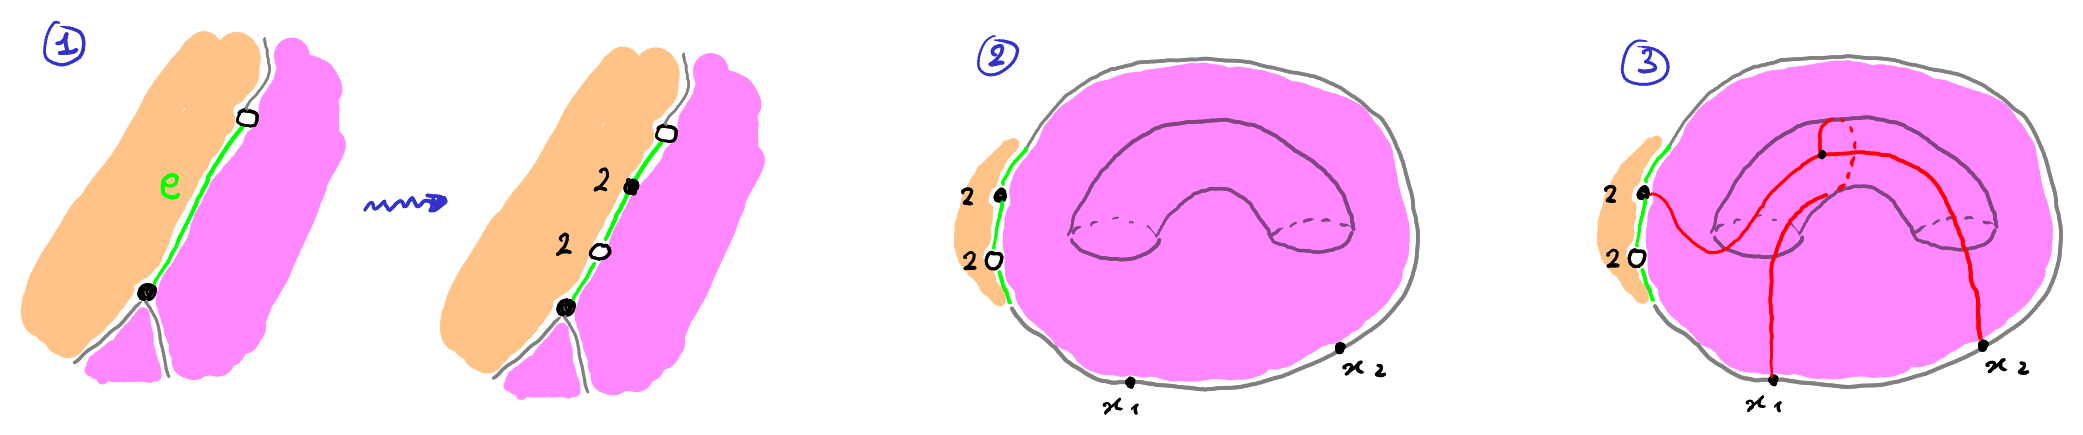
\includegraphics[width=.9\textwidth]{move4-2}
\end{center}
After these operations, we get a new \dessin{} $\Gamma$. It's easy to check that $\Gamma$ realizes the candidate datum $\mathcal{D}$.\qedhere
\end{manycases}
\end{proof}

\begin{combinatorialmove}\label{move:33-22}
Let $\mathcal{D}=\datum{\Sigma_g,d}{\pi_1,\pi_2,[s,d-s]}$ be a proper candidate datum. Assume that:
\begin{enumerate}
\item $3\le s\le d-3$;
\item $g\ge 1$;
\item $[x,y]\subs\pi_1$ for some $x\ge 3$, $y\ge 3$;
\item $[2,2]\subs\pi_2$.
\end{enumerate}
Consider the partitions
\begin{align*}
\pi_1'=\pi_1\setminus[x,y]\cup[x-2,y-2],&&\pi_2'=\pi_2\setminus[2,2].
\end{align*}
Then
\[
\mathcal{D}'=\datum{\Sigma_{g-1},d-4}{\pi_1',\pi_2',[s-2,d-s-2]}
\]
is a proper candidate datum and $\mathcal{D}\cmove\mathcal{D}'$.
\end{combinatorialmove}
\begin{proof}
Consider a \dessin{} $\Gamma'$ realizing $\mathcal{D}'$. There are two cases.
\begin{manycases}[Case \arabic*:]
\case the vertex labeled $x-2$ touches the orange disk and the vertex labeled $y-2$ touches the pink disk (or vice versa). Then we perform the following operations.
\begin{enumerate}
\item Attach a tube to $\Sigma_{g-1}$ with one endpoint in the orange disk and the other in the pink one.
\item Add two black vertices and two white vertices as shown in the picture.
\item Perform the joining operation along the red edges, replacing the black vertices labeled $x-2$, $2$ with a vertex of degree $x$, and the black vertices labeled $y-2$, $2$, with a vertex of degree $y$.
\end{enumerate}
\begin{center}
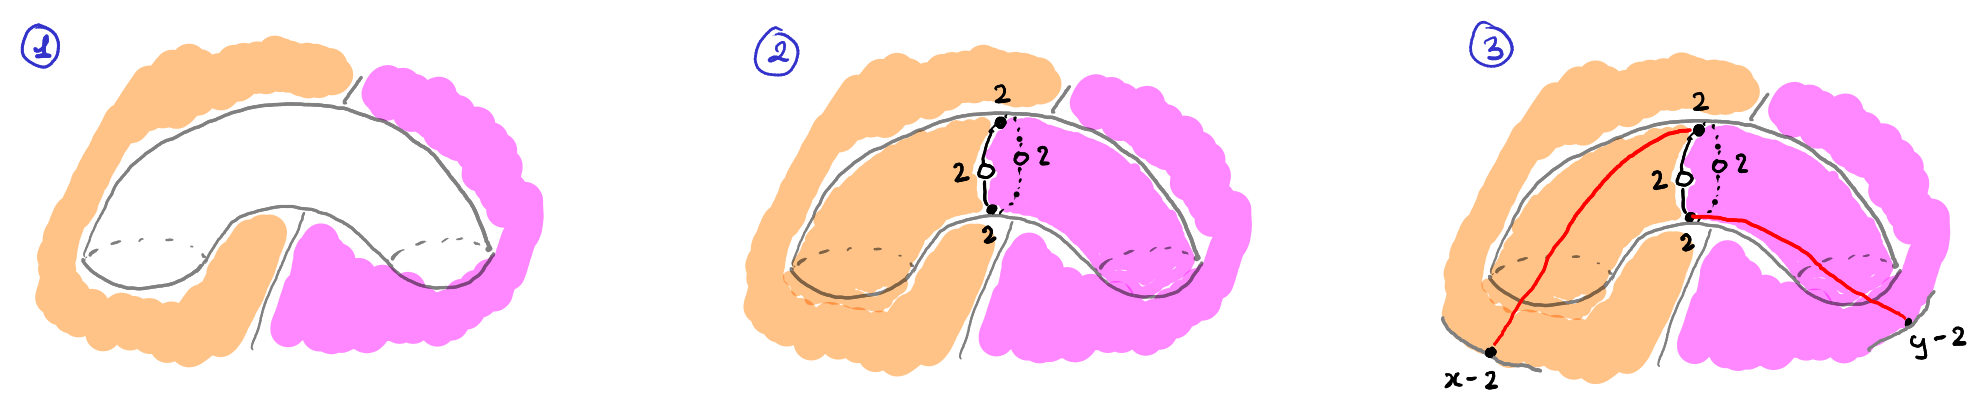
\includegraphics[width=.9\textwidth]{move5-1}
\end{center}
After these operations, we get a new \dessin{} $\Gamma$. It's easy to check that $\Gamma$ realizes the candidate datum $\mathcal{D}$.
\case both the vertices labeled $x-2$ and $y-2$ touch (say) the pink disk. Fix an edge $e$ of $\Gamma'$ that lies on the boundary of both disks. We perform the following operations.
\begin{enumerate}
\item Add two black vertex and two white vertex on $e$ as shown in the picture.
\item Attach a tube to $\Sigma_{g-1}$ with both endpoints in the pink disk.
\item Perform the joining operation along the red edges, replacing the black vertices labeled $x-2$, $2$ with a vertex of degree $x$, and the black vertices labeled $y-2$, $2$, with a vertex of degree $y$.
\end{enumerate}
\begin{center}
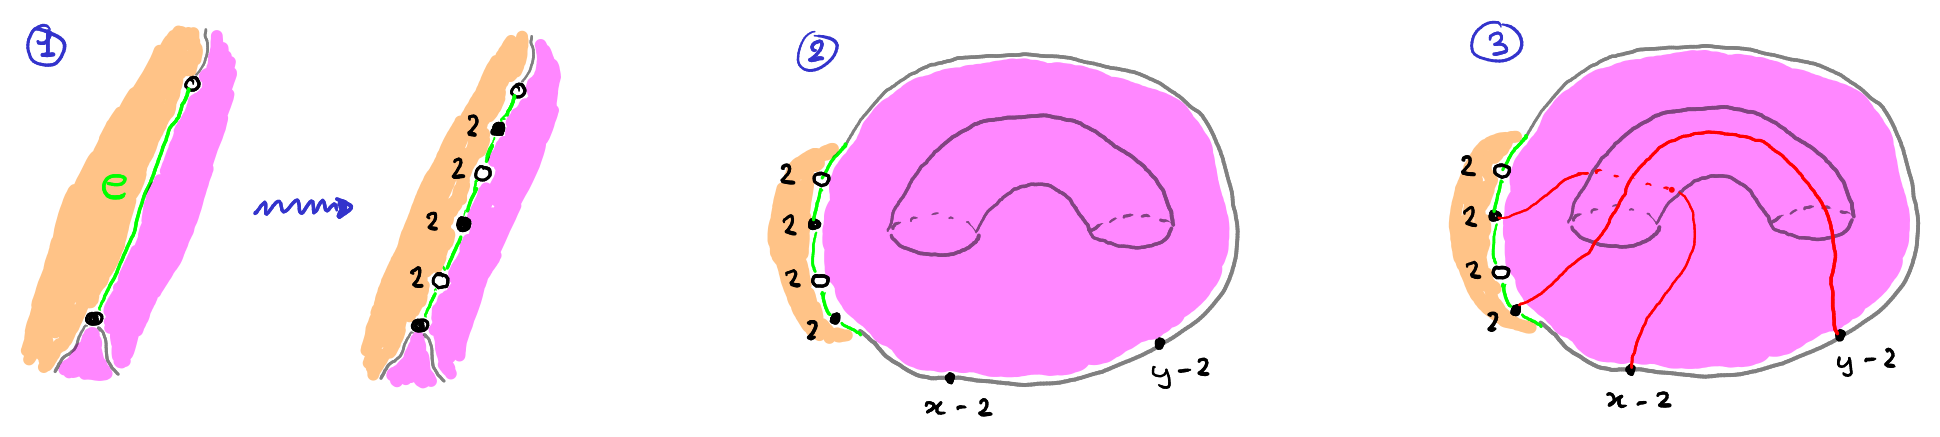
\includegraphics[width=.9\textwidth]{move5-2}
\end{center}
After these operations, we get a new \dessin{} $\Gamma$. It's easy to check that $\Gamma$ realizes the candidate datum $\mathcal{D}$.\qedhere
\end{manycases}
\end{proof}

\begin{combinatorialmove}\label{move:4-3}
Let $\mathcal{D}=\datum{\Sigma_g,d}{\pi_1,\pi_2,[s,d-s]}$ be a proper candidate datum. Assume that:
\begin{enumerate}
\item $2\le s\le d-2$;
\item $g\ge 1$;
\item there is an element $x\in\pi_1$ such that $x\ge 4$;
\item there is an element $y\in\pi_2$ such that $y\ge 3$.
\end{enumerate}
Consider the partitions
\begin{align*}
\pi_1'=\pi_1\setminus[x]\cup[x-2],&&\pi_2'=\pi_2\setminus[y]\cup[y-2].
\end{align*}
Then
\[
\mathcal{D'}=\datum{\Sigma_{g-1},d-2}{\pi_1',\pi_2',[s-1,d-s-1]}
\]
is a proper candidate datum and $\mathcal{D}\cmove\mathcal{D}'$.
\end{combinatorialmove}
\begin{proof}
Consider a \dessin{} $\Gamma'$ realizing $\mathcal{D}'$. There are two cases.
\begin{manycases}[Case \arabic*:]
\case the vertex labeled $x-2$ touches the orange disk and the vertex labeled $y-2$ touches the pink disk (or vice versa). Then we perform the following operations.
\begin{enumerate}
\item Attach a tube to $\Sigma_{g-1}$ with one endpoint in the orange disk and the other in the pink one.
\item Add one black vertex and one white vertex as shown in the picture.
\item Perform the joining operation along the red edges, replacing the black vertices labeled $x-2$, $2$ with a vertex of degree $x$, and the white vertices labeled $y-2$, $2$, with a vertex of degree $y$.
\end{enumerate}
\begin{center}
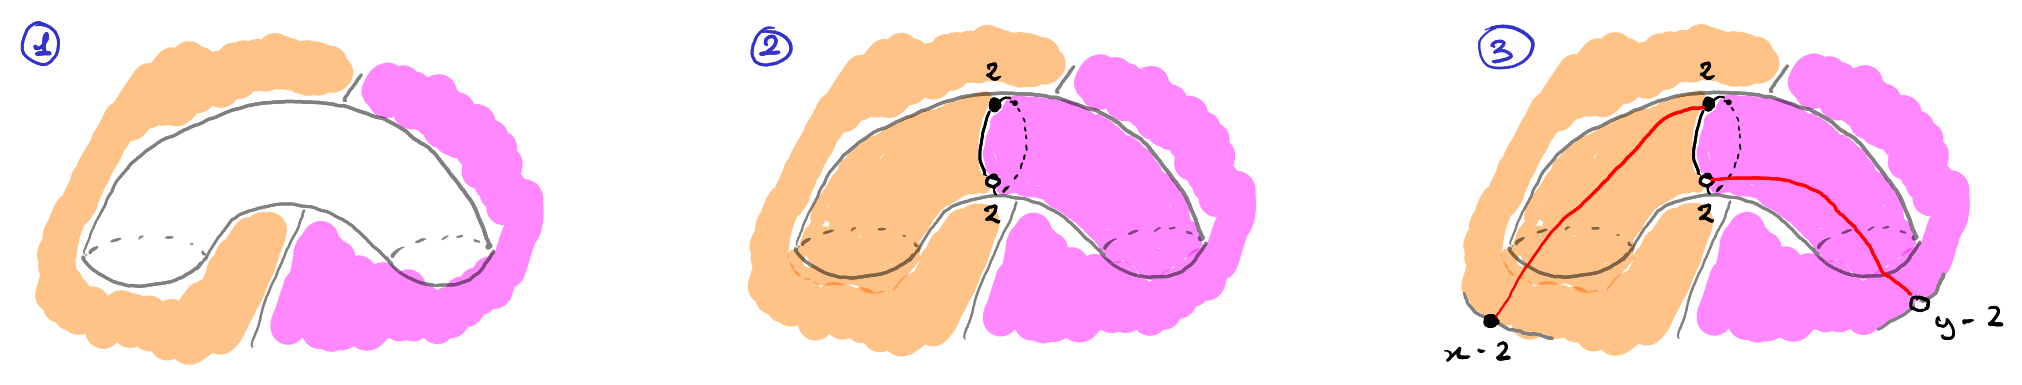
\includegraphics[width=.9\textwidth]{move6-1}
\end{center}
After these operations, we get a new \dessin{} $\Gamma$. It's easy to check that $\Gamma$ realizes the candidate datum $\mathcal{D}$.
\case let $u$ be the black vertex corresponding to $x-2$, and let $v$ be the white vertex corresponding to $y-2$; assume that neither $u$ nor $v$ touch (say) the orange disk. Analyzing this case will be a bit more involved. We start by coloring all the edges of $\Gamma'$  that lie on the boundary of both disks with the color green; our aim will be to prove that we can add two vertices of degree $2$ -- one white and one black -- on a green edge, in such a way that the vertices
\begin{center}
\begin{tikzpicture}
\foreach \i in {0,...,5} { \coordinate (\i) at (\i*2cm,0); }
\foreach \i [evaluate=\i as \ii using \i+1] in {0,...,4} \foreach \j in {1,2} { \coordinate (\i-\j) at ($\j/3*(\ii)+{1-\j/3}*(\i)$); }
\draw[gray] (0-2) -- (1-1) (3-2) -- (4-1);
\draw[gray,dashed] (0-1) -- (0-2) (1-1) -- (1-2) (3-1) -- (3-2) (4-1) -- (4-2);
\draw[green] (1-2) -- (3-1);
\foreach \i in {1,3} { \fill[black] (\i) circle(2pt); }
\foreach \i in {2,4} { \filldraw[black,fill=white] (\i) circle(2pt); }
\foreach \i/\l in {1/u,2/2,3/2,4/v} { \node[above=3pt] at (\i) {$\l$}; }
\end{tikzpicture}
\end{center}
appear in this order along the perimeter of the pink disk.

Let us unwind the perimeter of the pink disk in the shape of a circle. Some vertices may appear more than once, if they are traversed several times while traveling along the perimeter; for instance, $u$ appears $x-2\ge 2$ times, while $v$ appears $y-2$ times. Likewise, some edges may appear twice, with different orientations; this happens exactly for all the non-green edges on the boundary of the pink disk.
\begin{itemize}
\columnratio{.5}\setlength{\columnsep}{0em}
\item If $\{u,v,u,\text{green edge}\}$ appear in this order on the perimeter, then adding the two vertices on this green edge will give the desired result. The same holds if $\{v,u,v,\text{green edge}\}$ occur on the perimeter in this order.

\begin{center}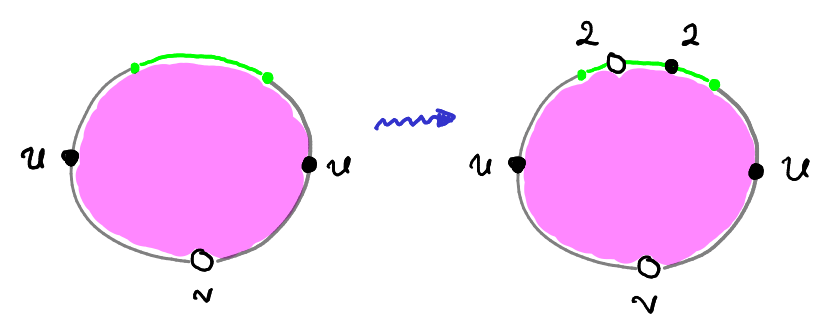
\includegraphics[width=.5\textwidth]{move6-2-1}\end{center}

\item Otherwise, consider the pictures below.
\begin{enumerate}
\item We are in the following situation: there is a portion of the perimeter that contains all of the appearances of $u$, and does not contain any appearance of $v$ or any green edge; the same holds if we swap the roles of $u$ and $v$. Notice that $u$ and $v$ are never adjacent to a green edge, since by assumption they do not touch the orange disk.
\item Consider the first (leftmost in the picture) occurrence of $u$ on the perimeter, and let $\alpha$ be the edge immediately afterwards. Since $\alpha$ is not a green edge, it must occur somewhere else on the perimeter, with the opposite orientation; notice that it cannot occur immediately before the first occurrence of $u$, otherwise $u$ would have degree $1$, therefore it will occur somewhere to the right.
\item Consider now the first (rightmost in the picture) occurrence of $v$, and let $\beta$ be the edge immediately before. Since $\beta$ is not a green edge, it will also occur somewhere else to the left.
\item Let $a$ be the other endpoint of $\alpha$, and let $b$ be the other endpoint of $\beta$. We erase the edges $\alpha$ and $\beta$ and add two new edges, connecting $u$ to $v$ and $a$ to $b$ as shown in the picture.
\item It's now easy to see that the pink region is still a disk, and that the length of the perimeter has not changed. Moreover, traveling along the perimeter, we encounter $\{u,v,u\}$ in this order, without any green edges in between. Since there must be at least a green edge on the perimeter, the argument of the first bullet point applies.
\end{enumerate}
\begin{center}
\newcommand{\pic}[1]{\raisebox{-1.\height}{\includegraphics[width=.28\linewidth]{#1}}}
\pic{move6-2-2-1}\qquad\pic{move6-2-2-2}\qquad\pic{move6-2-2-3}\\
\bigskip
\pic{move6-2-2-4}\qquad\pic{move6-2-2-5}
\end{center}
\end{itemize}
Once we have added the two vertices of degree 2 as shown above, we can perform the following operations.
\begin{enumerate}
\item Attach a tube to $\Sigma_{g-1}$ with both endpoints in the pink disk.
\item Perform the joining operation along the red edges, replacing the black vertices labeled $u$, $2$ with a vertex of degree $x$, and the white vertices labeled $v$, $2$, with a vertex of degree $y$.
\end{enumerate}
\begin{center}
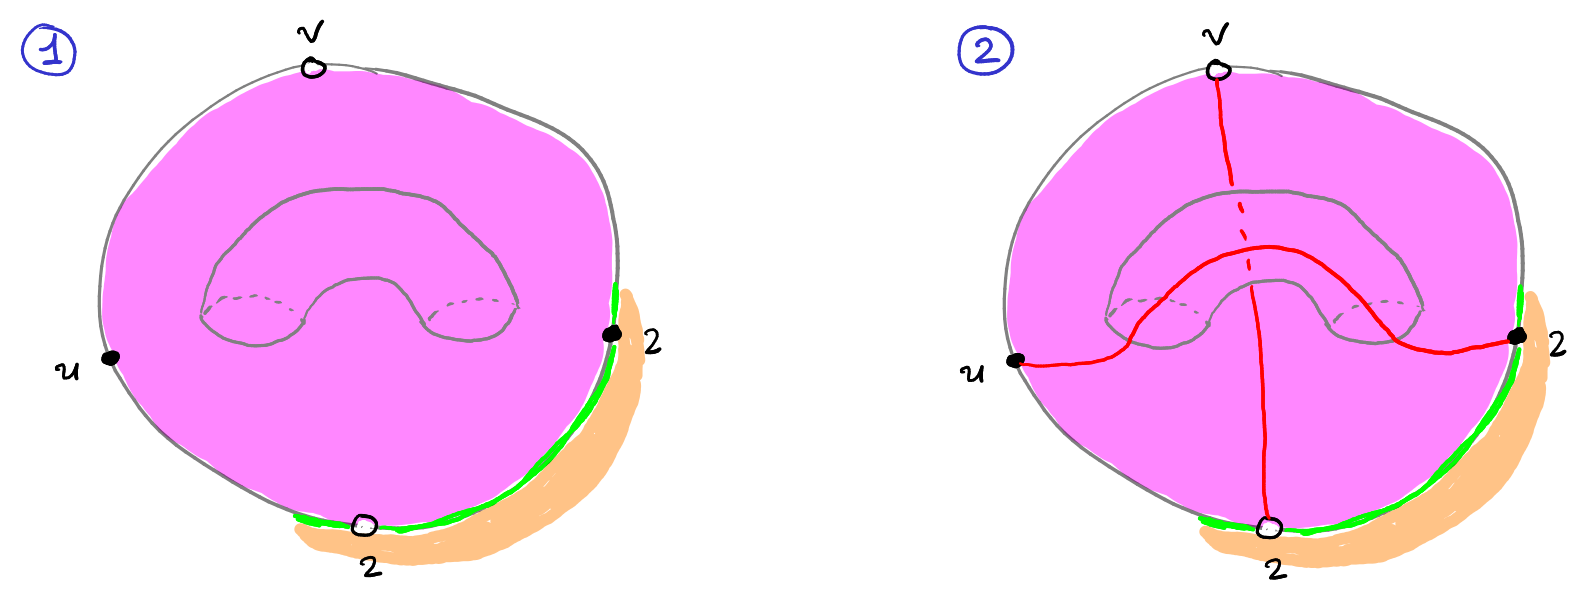
\includegraphics[width=.6\textwidth]{move6-2}
\end{center}
After these operations, we get a new \dessin{} $\Gamma$. It's easy to check that $\Gamma$ realizes the candidate datum $\mathcal{D}$.\qedhere
\end{manycases}
\end{proof}

\section{Exceptional data}
In this section, we will give a complete list of the proper exceptional candidate data of the form
\[
\datum{\Sigma_g,d}{\pi_1,\pi_2,[s,d-s]}.
\]

\begin{theorem}\label{th:exceptional-n3-g0}
Let $\mathcal{D}=\datum{\Sigma_0,d}{\pi_1,\pi_2,[s,d-s]}$ be a proper candidate datum. Then $\mathcal{D}$ is realizable unless it satisfies one of the following.
\begin{enumerate}
\item $\mathcal{D}=\datum{\Sigma_0,12}{[2,2,2,2,2,2],[1,1,1,3,3,3],[6,6]}$.
\item $\mathcal{D}=\datum{\Sigma_0,2k}{[2,\ldots,2],[2,\ldots,2],[s,2k-s]}$ with $k\ge 2$, $s\neq k$.
\item $\mathcal{D}=\datum{\Sigma_0,2k}{[2,\ldots,2],[1,2,\ldots,2,3],[k,k]}$ with $k\ge2$.
\item $\mathcal{D}=\datum{\Sigma_0,4k+2}{[2,\ldots,2],[1,\ldots,1,k+1,k+2],[2k+1,2k+1]}$ with $k\ge 1$.
\item $\mathcal{D}=\datum{\Sigma_0,4k}{[2,\ldots,2],[1,\ldots,1,k+1,k+1],[2k-1,2k+1]}$ with $k\ge2$.
\item $\mathcal{D}=\datum{\Sigma_0,kh}{[h,\ldots,h],[1,\ldots,1,k+1],[lk,(h-l)k]}$ with $h\ge 2$, $k\ge 2$, $1\le l<h$.
\end{enumerate}
\end{theorem}

\begin{lemma}\label{th:exceptional-n3-s1}
Let $\mathcal{D}=\datum{\Sigma_g,d}{\pi_1,\pi_2,[1,d-1]}$ be a proper candidate datum. Then $\mathcal{D}$ is realizable unless
\[
\mathcal{D}=\datum{\Sigma_0,2k}{[2,\ldots,2],[2,\ldots,2],[1,2k-1]}
\]
for some $k\ge 2$.
\end{lemma}
\begin{proof}
If $g=0$ the claim is a corollary of \cref{th:exceptional-n3-g0}. We then proceed by induction on $g\ge 1$. The Riemann-Hurwitz condition \eqref{eq:rh-n3} immediately implies that one of the partitions, say $\pi_1$, contains an element $x\ge 3$. By applying \cref{move:s1-3}, we can reduce the problem to the realizability of the candidate datum
\[
\mathcal{D}'=\datum{\Sigma_{g-1},d}{\pi_1\setminus[x]\cup[1,1,x-2],\pi_2,[1,d-1]},
\]
which is realizable by induction.
\end{proof}

\begin{theorem}\label{th:exceptional-n3-g1}
Let $\mathcal{D}=\datum{\Sigma_1,d}{\pi_1,\pi_2,[s,d-s]}$ be a proper candidate datum. Then $\mathcal{D}$ is realizable unless it satisfies one of the following.
\begin{enumerate}
\item $\mathcal{D}=\datum{\Sigma_1,6}{[3,3],[3,3],[2,4]}$.
\item $\mathcal{D}=\datum{\Sigma_1,8}{[2,2,2,2],[4,4],[3,5]}$.
\item $\mathcal{D}=\datum{\Sigma_1,12}{[2,2,2,2,2,2],[3,3,3,3],[5,7]}$.
\item $\mathcal{D}=\datum{\Sigma_1,16}{[2,2,2,2,2,2,2,2],[1,3,3,3,3,3],[8,8]}$.
\item $\mathcal{D}=\datum{\Sigma_1,2k}{[2,\ldots,2],[2,\ldots,2,3,5],[k,k]}$ with $k\ge 5$.
\end{enumerate}
\end{theorem}
\begin{proof}
Thanks to \cref{th:exceptional-n3-s1} we can assume that $2\le s\le d-2$. We analyze several cases.
\begin{manycases}
\case Assume that $d\le 14$. Using Zheng's algorithm, a list of all the proper exceptional candidate data has been computed. It turns out that $\mathcal{D}$ is realizable unless one of the following holds.
\begin{enumerate}
\item $\mathcal{D}=\datum{\Sigma_1,6}{[3, 3],[3, 3],[2, 4]}$.
\item $\mathcal{D}=\datum{\Sigma_1,8}{[2, 2, 2, 2],[4, 4],[3, 5]}$.
\item $\mathcal{D}=\datum{\Sigma_1,10}{[2, 2, 2, 2, 2],[2, 3, 5],[5, 5]}$.
\item $\mathcal{D}=\datum{\Sigma_1,12}{[2, 2, 2, 2, 2, 2],[3, 3, 3, 3],[5, 7]}$.
\item $\mathcal{D}=\datum{\Sigma_1,12}{[2, 2, 2, 2, 2, 2],[2, 2, 3, 5],[6, 6]}$.
\item $\mathcal{D}=\datum{\Sigma_1,14}{[2, 2, 2, 2, 2, 2, 2],[2, 2, 2, 3, 5],[7, 7]}$.
\end{enumerate}
This is in agreement with the theorem statement.

\case Assume that:
\begin{enumerate}
\item there is an element $x\in\pi_1$ such that $x\ge 4$;
\item $2\in\pi_2$;
\item $\pi_2\neq[2,\ldots,2]$.
\end{enumerate}
By applying \cref{move:4-2}, we can reduce the problem to the realizablility of the candidate datum
\[
\mathcal{D}'=\datum{\Sigma_0,d-2}{\pi_1',\pi_2',[s-1,d-s-1]},
\]
where $\pi_1'=\pi_1\setminus[x]\cup[1,x-3]$ and $\pi_2'=\pi_2\setminus[2]$. Notice that $\pi_1'$ and $\pi_2'$ are both different from $[2,\ldots,2]$. Therefore, by \cref{th:exceptional-n3-g0}, $\mathcal{D}'$ is realizable unless
\begin{align*}
\pi_1'=[1,\ldots,1,k+1],&&\pi_2'=[h,\ldots,h]
\end{align*}
for some $k\ge 2$, $h\ge 3$.
If this is the case, then one of the following must hold.
\begin{itemize}
\item $\pi_1=[1,\ldots,1,k+4]$ and $\pi_2=[2,h,\ldots,h]$. Then we can apply \cref{move:4-2} and reduce to
\[
\mathcal{D}\cmove\datum{\Sigma_0,d-2}{[1,\ldots,1,2,k],[h,\ldots,h],[s-1,d-s-1]},
\]
which is realizable by \cref{th:exceptional-n3-g0}.
\item $\pi_1=[1,\ldots,1,4,k+1]$ and $\pi_2=[2,h,\ldots,h]$. Then we can apply \cref{move:4-3} and reduce to
\[
\mathcal{D}\cmove\datum{\Sigma_0,d-2}{[1,\ldots,1,2,k+1],[2,h-2,h,\ldots,h],[s-1,d-s-1]},
\]
which is realizable by \cref{th:exceptional-n3-g0}.
\end{itemize}

\case Assume that:
\begin{enumerate}
\item there is an element $x\in\pi_1$ such that $x\ge 4$;
\item there is an element $y\in\pi_2$ such that $y\ge 4$.
\end{enumerate}
We can further assume that $2\not\in\pi_1$, $2\not\in\pi_2$, otherwise we are done by case \caseref{2}. By applying \cref{move:4-3}, we can reduce the problem to the realizability of the candidate datum
\[
\mathcal{D}'=\datum{\Sigma_0,d-2}{\pi_1',\pi_2',[s-1,d-s-2]},
\]
where $\pi_1'=\pi_1\setminus[x]\cup[x-2]$ and $\pi_2'=\pi_2\setminus[y]\cup[y-2]$. Notice that $\pi_1'$ and $\pi_2'$ are bot different from $[2,\ldots,2]$ (unless one of them is equal to $[2]$, but then $\mathcal{D}'$ would be realizable anyway). Therefore, by \cref{th:exceptional-n3-g0}, $\mathcal{D}'$ is realizable, unless, without loss of generality,
\begin{align*}
\pi_1'=[1,\ldots,1,k+1],&&\pi_2'=[h,\ldots,h]
\end{align*}
for some $k\ge 2$, $h\ge 3$. If this is the case, then $\pi_1=[1,\ldots,1,k+3]$ and $\pi_2=[h,\ldots,h+2]$, but then we can apply \cref{move:4-3} and reduce to
\[
\mathcal{D}\cmove\datum{\Sigma_2,d-2}{[1,\ldots,1,k+1],[h-2,h,\ldots,h,h+2],[s-1,d-s-1]},
\]
which is realizable by \cref{th:exceptional-n3-g0}.

\case Assume that:
\begin{enumerate}
\item there is an element $x\in\pi_1$ such that $x\ge 4$;
\item $3\in\pi_2$.
\end{enumerate}
We can further assume that $2\not\in\pi_2$, otherwise we are done by case \caseref{2}, and that $\max(\pi_2)=3$, otherwise we are done by case \caseref{3}. By applying \cref{move:4-3}, we can reduce the problem to the realizability of the candidate datum
\[
\mathcal{D}'=\datum{\Sigma_0,d-2}{\pi_1',\pi_2',[s-1,d-s-1]},
\]
where $\pi_1'=\pi_1\setminus[x]\cup[x-2]$ and $\pi_2'=\pi_2\setminus[3]\cup[1]$. By \cref{th:exceptional-n3-g0}, $\mathcal{D}'$ is realizable unless one of the following holds.
\begin{itemize}
\item $\mathcal{D}'=\datum{\Sigma_0,12}{[2,2,2,2,2,2],[1,1,1,3,3,3],[6,6]}$. In this case $d=14$, so we are done by case \caseref{1}.
\item $\mathcal{D}'=\datum{\Sigma_0,4}{[2,2],[1,3],[2,2]}$. In this case $d=6$, so we are done by case \caseref{1}.
\item $\mathcal{D}'=\datum{\Sigma_0,8}{[2,2,2,2],[1,1,3,3],[3,5]}$. In this case $d=10$, so we are done by case \caseref{1}.
\item $\mathcal{D}'=\datum{\Sigma_0,2h}{[h,h],[1,\ldots,1,3],[2l,2(h-l)]}$ for some $h\ge 2$, $1\le l<h$. In this case $\pi_1=[h,h+2]$ and $\pi_2=[1,\ldots,1,3,3]$. If $d\le 7$ we are done by case \caseref{1}. Otherwise $[1,1,3]\subs\pi_2$, therefore we can apply \cref{move:113} and reduce to
\[
\mathcal{D}\cmove\datum{\Sigma_0,2h+2}{[h,h+2],[1,\ldots,1,3],[s,2h+2-s]},
\]
which is realizable by \cref{th:exceptional-n3-g0}.
\end{itemize}

\case Assume that:
\begin{enumerate}
\item $3\in\pi_1$;
\item $\pi_2\neq[2,\ldots,2]$.
\end{enumerate}
We can further assume that $\max(\pi_1)=3$ and $\max(\pi_2)\le 3$, otherwise the situation is already covered by cases \caseref{2}, \caseref{3} and \caseref{4}. We analyze different sub-cases.
\begin{manycases}[Case \thecasei.\arabic*:]
\case $[1,1]\subs\pi_1$. By \cref{move:113} we have
\[
\mathcal{D}\cmove\datum{\Sigma_0,d}{\pi_1\setminus[3]\cup[1,1,1],\pi_2,[s,d-s]},
\]
which is realizable by \cref{th:exceptional-n3-g0}.
\case $[3,3]\subs\pi_1$ and $[2,2]\subs\pi_2$. If $s=2$ or $s=d-2$ then $\mathcal{D}$ is realizable by \cref{move:s2-23-22}. Otherwise, by \cref{move:33-22} we have
\[
\mathcal{D}\cmove\datum{\Sigma_0,d-4}{\pi_1\setminus[3,3]\cup[1,1],\pi_2\setminus[2,2],[s-2,d-s-2]},
\]
which is realizable by \cref{th:exceptional-n3-g0} unless $\pi_1=[1,3,3,3]$ and $\pi_2=[2,2,3,3]$. If this is the case, then we are done by case \caseref{1}, since $d=10$.
\case $[2,2]\not\subs\pi_2$. The Riemann-Hurwitz condition \eqref{eq:rh-n3} immediately implies that $3\in\pi_2$. We can assume that $d\ge 13$, otherwise we are done by case \caseref{1}. Assume by contradiction that $\mathcal{D}$ is not realizable. Then $[1,1]\not\subs\pi_2$ (case \caseref{5.1}), but then $[3,3]\subs\pi_2$. It follows (case \caseref{5.2}) that $[2,2]\not\subs\pi_1$; moreover, case \caseref{5.1} also implies that $[1,1]\not\subs\pi_1$. In other words, both $\pi_1$ and $\pi_2$ can be written as $\rho\cup[3,\ldots,3]$, where $\rho\subs[1,2]$  (possibly different for $\pi_1$ and $\pi_2$). As a consequence, we have the inequalities
\begin{align*}
d\ge 3\card{\pi_1}-3,&&d\ge 3\card{\pi_2}-3,
\end{align*}
which contradict the Riemann-Hurwitz condition \eqref{eq:rh-n3} if $d\ge 13$.
\case $[3,3]\not\subs\pi_1$. From the Riemann-Hurwitz condition \eqref{eq:rh-n3} it follows that $[3,3]\subs\pi_2$, but then $\mathcal{D}$ is realizable by cases \caseref{5.2} and \caseref{5.3}.
\end{manycases}

\case Assume that:
\begin{enumerate}
\item $\max(\pi_1)\ge 4$;
\item $\pi_2=[2,\ldots,2]$.
\end{enumerate}
Let $x=\max(\pi_1)$. By applying \cref{move:4-2}, we can reduce the problem to the realizability of the candidate datum
\[
\mathcal{D'}=\datum{\Sigma_0,d-2}{\pi_1\setminus[x]\cup[1,x-3],[2,\ldots,2],[s-1,d-s-1]},
\]
which is realizable by \cref{th:exceptional-n3-g0} unless one of the following holds.
\begin{itemize}
\item $\mathcal{D}=\datum{\Sigma_1,14}{\pi_1,[2,\ldots,2],[s,14-s]}$. In this case $d=14$, so we are done by case \caseref{1}.
\item $\mathcal{D}=\datum{\Sigma_1,2k+2}{[2,\ldots,2,3,5],[2,\ldots,2],[k+1,k+1]}$ with $k\ge 2$. If $k=2$ or $k=3$ then we are done by case \caseref{1}, otherwise this datum is in fact one of the exceptions listed in the statement of the theorem.
\item $\mathcal{D}=\datum{\Sigma_1,2k+2}{[2,\ldots,2,6],[2,\ldots,2],[k+1,k+1]}$ with $k\ge 2$. By \cref{move:4-2} we have
\[
\mathcal{D}\cmove\datum{\Sigma_0,2k}{[2,\ldots,2],[2,\ldots,2],[k,k]},
\]
which is realizable by \cref{th:exceptional-n3-g0}.
\item $\mathcal{D}=\datum{\Sigma_1,4k+4}{[1,\ldots,1,k+1,k+2,4],[2,\ldots,2],[2k+2,2k+2]}$ with $k\in\{1,2\}$. In this case $d\le 12$, so we are done by case \caseref{1}.
\item $\mathcal{D}=\datum{\Sigma_1,4k+4}{[1,\ldots,1,k+2,k+4],[2,\ldots,2],[2k+2,2k+2]}$ with $k\ge 1$. If $k=1$ then $d=8$, so we are done by case \caseref{1}. Otherwise, by \cref{move:4-2} we have
\[
\mathcal{D}\cmove\datum{\Sigma_0,4k+2}{[1,\ldots,1,2,k,k+2],[2,\ldots,2],[2k+1,2k+1]},
\]
which is realizable for $k\ge 2$ by \cref{th:exceptional-n3-g0}.
\item $\mathcal{D}=\datum{\Sigma_1,4k+4}{[1,\ldots,1,k+1,k+5],[2,\ldots,2],[2k+2,2k+2]}$ with $k\ge 1$. By \cref{move:4-2} we have
\[
\mathcal{D}\cmove\datum{\Sigma_0,4k+2}{[1,\ldots,1,2,k+1,k+1],[2,\ldots,2],[2k+1,2k+1]},
\]
which is realizable by \cref{th:exceptional-n3-g0} (even if $k=1$).
\item $\mathcal{D}=\datum{\Sigma_1,4k+2}{[1,\ldots,1,k+1,k+1,4],[2,\ldots,2],[2k,2k+2]}$ with $k\in\{2,3\}$. In this case $d\le 14$, so we are done by case \caseref{1}.
\item $\mathcal{D}=\datum{\Sigma_1,4k+2}{[1,\ldots,1,k+1,k+4],[2,\ldots,2],[2k,2k+2]}$ with $k\ge 2$. If $k=2$ then $d=10$, so we are done by case \caseref{1}. Otherwise, by \cref{move:4-2} we have
\[
\mathcal{D}\cmove\datum{\Sigma_0,4k}{[1,\ldots,1,2,k,k+1],[2,\ldots,2],[2k-1,2k+1]},
\]
which is realizable for $k\ge 3$ by \cref{th:exceptional-n3-g0}.
\item $\mathcal{D}=\datum{\Sigma_1,2k+2}{[1,\ldots,1,k+1,4],[2,\ldots,2],[k+1,k+1]}$ with $k\in\{2,3\}$. In this case $d\le 8$, so we are done by case \caseref{1}.
\item $\mathcal{D}=\datum{\Sigma_1,2k+2}{[1,\ldots,1,k+4],[2,\ldots,2],[k+1,k+1]}$ with $k\ge 2$. If $k=2$ or $k=3$ then $d\le 8$, so we are done by case \caseref{1}. Otherwise, by \cref{move:4-2} we have
\[
\mathcal{D}\cmove\datum{\Sigma_0,2k}{[1,\ldots,1,2,k],[2,\ldots,2],[k,k]},
\]
which is realizable for $k\ge 4$ by \cref{th:exceptional-n3-g0}.
\end{itemize}

\case Assume that:
\begin{enumerate}
\item $\max(\pi_1)=3$;
\item $\pi_2=[2,\ldots,2]$.
\end{enumerate}
The Riemann-Hurwitz condition \eqref{eq:rh-n3} immediately implies that $[3,3,3,3]\subs\pi_1$. If $s=2$ or $s=d-2$ then $\mathcal{D}$ is realizable by \cref{move:s2-23-22}. Otherwise, by \cref{move:33-22} we have
\[
\mathcal{D}\cmove\datum{\Sigma_0,d-4}{\pi_1\setminus[3,3]\cup[1,1],[2,\ldots,2],[s-2,d-s-2]},
\]
which is realizable by \cref{th:exceptional-n3-g0} unless one of the following holds.
\begin{itemize}
\item $\mathcal{D}=\datum{\Sigma_1,16}{[1,3,3,3,3,3],[2,2,2,2,2,2,2,2],[8,8]}$. This is in fact one of the exceptions listed in the statement.
\item $\mathcal{D}=\datum{\Sigma_1,12}{[3,3,3,3,3],[2,2,2,2,2,2],[5,7]}$. This is in fact one of the exceptions listed in the statement.
\end{itemize}
\end{manycases}
The cases we have analyzed (up to swapping $\pi_1$ and $\pi_2$) cover all the proper candidate data of the form $\datum{\Sigma_1,d}{\pi_1,\pi_2,[s,d-s]}$. We have showed that every datum that is not listed in the statement is realizable, therefore the proof is complete.
\end{proof}

\begin{lemma}\label{th:exceptional-n3-special-family}
Let $\mathcal{D}=\datum{\Sigma_g,d}{\pi_1,\pi_2,[s,d-s]}$ be a proper candidate datum. Assume that:
\begin{enumerate}
\item $g\ge 2$;
\item $\pi_1=\rho_1\cup[3,\ldots,3]$ for some $\rho_1\subs[1,2]$;
\item $\pi_2=\rho_2\cup[3,\ldots,3]$ for some $\rho_2\subs[1,2]$.
\end{enumerate}
Then $\mathcal{D}$ is realizable.
\end{lemma}
\begin{proof}
\newcommand{\env}[1]{\underline{#1}}
In the scope of this proof, we define an \emph{augmented combinatorial datum} as a combinatorial datum
\[
\mathcal{D}=\datum{\Sigma_g,d}{\pi_1,\pi_2,\pi_3}
\]
where some distinguished elements of $\pi_3$ are called \emph{enveloping}; we will underline the enveloping elements in order to recognize them. An augmented combinatorial datum is \emph{realizable} if it admits a \dessin{} $\Gamma$ such that, for every disk $D$ of the complement $\Sigma_g\setminus\Gamma$ that corresponds to an enveloping element of $\pi_3$, there is an edge of $\Gamma$ that does not lie on the boundary of any disk other than $D$; we say that such an edge is \emph{enveloped} by $D$.
\begin{manycases}[Step \arabic*.]
\case The augmented datum
\[
\mathcal{D}=\datum{\Sigma_2,12}{[3,3,3,3],[3,3,3,3],\pi_3}
\]
is realizable for $\pi_3\in\left\{[1,\env{11}],[2,\env{10}],[\env{3},\env{9}],[\env{4},\env{8}],[\env{5},\env{7}],[\env{6},\env{6}]\right\}$. The following picture presents realizations of these augmented data (as usual, we use the color orange for the disk associated to the first element of $\pi_3$ and the color pink for the other one).
\begin{center}
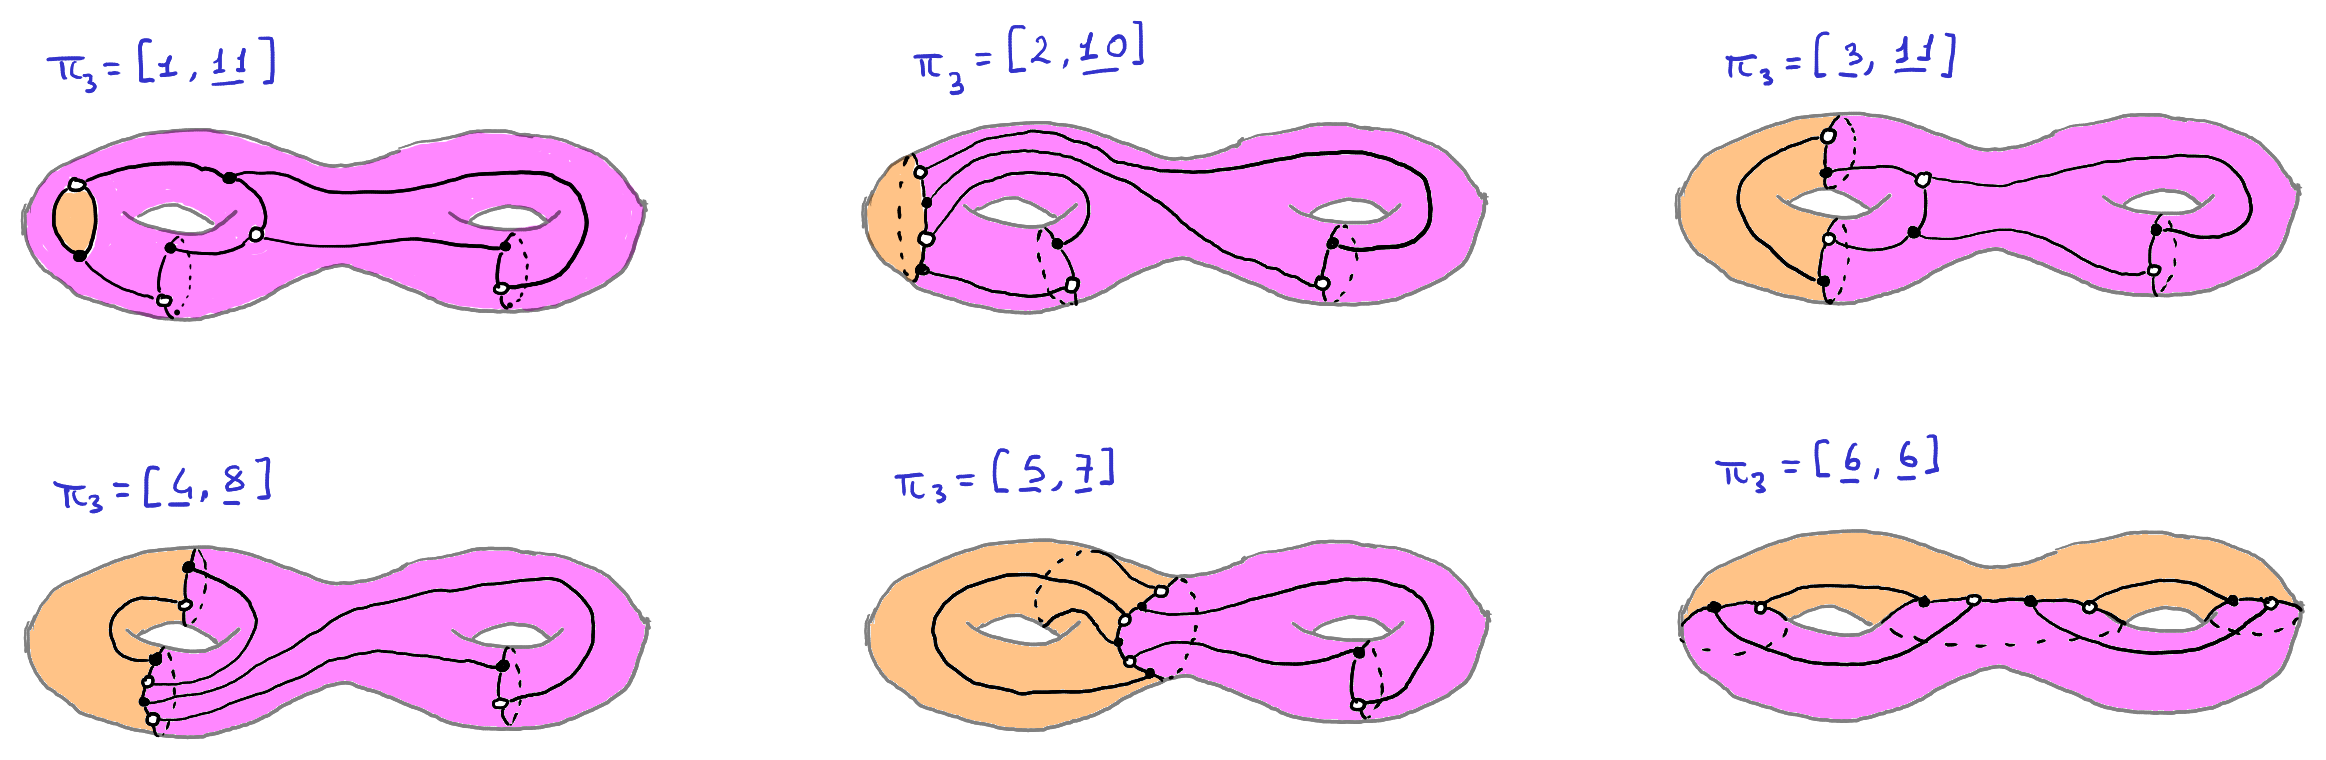
\includegraphics[width=.9\textwidth]{special-family-1}
\end{center}

\case Let $\mathcal{D}=\datum{\Sigma_g,d}{\pi_1,\pi_2,\pi_3}$ be an augmented realizable datum, and let $\env{x}\in\pi_3$ be an enveloping element. Then the augmented datum
\[
\mathcal{D}'=\datum{\Sigma_{g+1},d+6}{\pi_1\cup[3,3],\pi_2\cup[3,3],\pi_3\setminus[\env{x}]\cup[\env{x+6}]}
\]
is realizable. In fact, consider a \dessin{} $\Gamma$ realizing $\mathcal{D}$, and fix an edge $e$ enveloped by the disk associated to $\env{x}$. We perform the following operations.
\begin{enumerate}
\item Add one black vertex and one white vertex on $e$ as shown in the picture.
\item Attach a tube to $\Sigma_g$ close to $e$ and place two more vertices on this tube, as shown in the picture.
\item Draw two more arcs as shown in the picture.
\end{enumerate}
\begin{center}
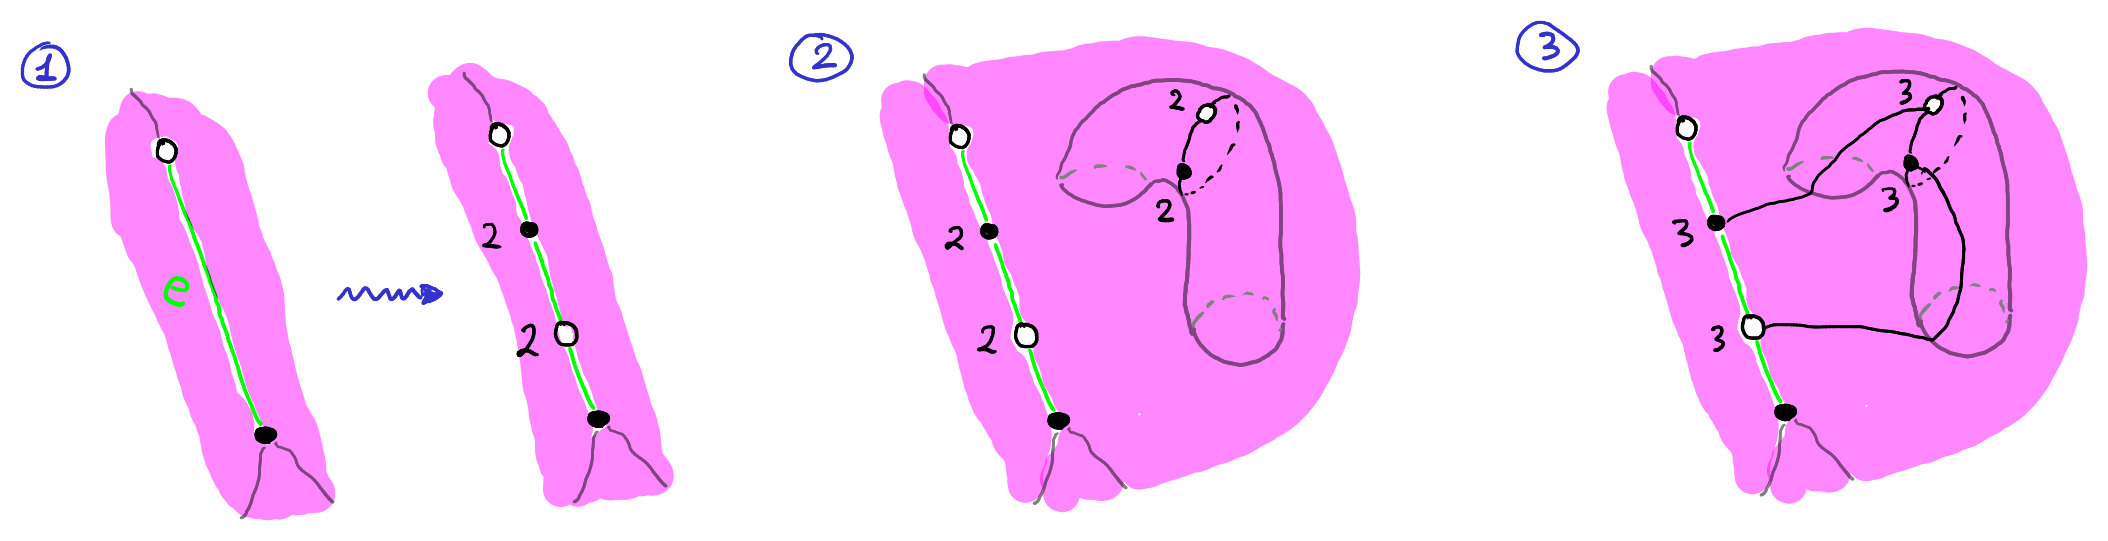
\includegraphics[width=.9\textwidth]{special-family-2}
\end{center}
After these operations we get a new \dessin{} $\Gamma'$. It's easy to check that $\Gamma'$ realizes the augmented datum $\mathcal{D}'$.

\case For every $g\ge 2$, the augmented datum
\[
\mathcal{D}=\datum{\Sigma_g,6g}{[3,\ldots,3],[3,\ldots,3],\pi_3}
\]
is realizable for $\pi_3\in\{[1,\env{6g-1}],[2,\env{6g-2}]\}\cup\{[\env{s},\env{6g-s}]:3\le s\le 3g\}$. This can be easily shown by induction on $g$ using step \caseref{1} for the base case and step \caseref{2} for the induction step.

\case[Step \arabic*.][sidebyside,sidebyside gap=2em,lower separated=false,lefthand width=.7\linewidth]
Let $\mathcal{D}=\datum{\Sigma_g,d}{\pi_1,\pi_2,\pi_3}$ be an augmented realizable datum, and let $\env{x}\in\pi_3$ be an enveloping element. Then the augmented datum
\[
\mathcal{D}'=\datum{\Sigma_g,d+2}{\pi_1\cup[2],\pi_2\cup[2],\pi_3\setminus[\env{x}]\cup[\env{x+2}]}
\]
is realizable. In fact, consider a \dessin{} $\Gamma$ realizing $\mathcal{D}$, and fix an edge $e$ enveloped by the disk associated to $\env{x}$. Then add one black vertex and one white vertex on $e$ as shown in the picture. The new \dessin{} realizes the augmented datum $\mathcal{D'}$.
\tcblower
\begin{center}
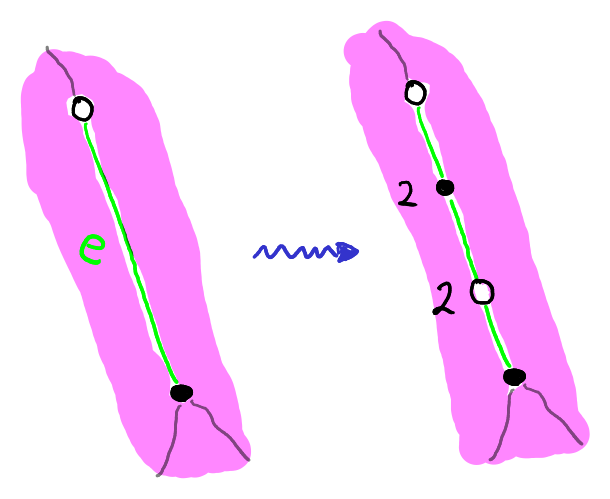
\includegraphics[width=\linewidth]{special-family-3}
\end{center}

\case[Step \arabic*.][sidebyside,sidebyside gap=2em,lower separated=false,lefthand width=.7\linewidth]
Let $\mathcal{D}=\datum{\Sigma_g,d}{\pi_1,\pi_2,\pi_3}$ be an augmented realizable datum, and let $\env{x}\in\pi_3$ be an enveloping element. Then the augmented datum
\[
\mathcal{D}'=\datum{\Sigma_g,d+3}{\pi_1\cup[3],\pi_2\cup[1,2],\pi_3\setminus[\env{x}]\cup[\env{x+3}]}
\]
is realizable. In fact, consider a \dessin{} $\Gamma$ realizing $\mathcal{D}$, and fix an edge $e$ enveloped by the disk associated to $\env{x}$. Then add one black vertex and two white vertices as shown in the picture. The new \dessin{} realizes the augmented datum $\mathcal{D'}$.
\tcblower
\begin{center}
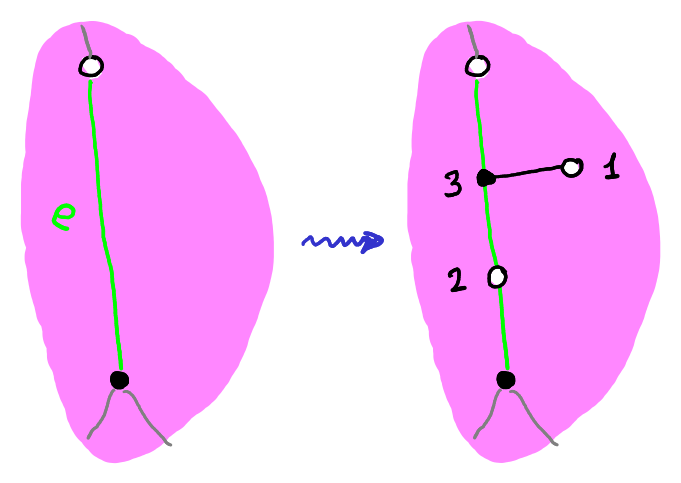
\includegraphics[width=\linewidth]{special-family-4}
\end{center}

\case[Step \arabic*.][sidebyside,sidebyside gap=2em,lower separated=false,lefthand width=.7\linewidth]
Let $\mathcal{D}=\datum{\Sigma_g,d}{\pi_1,\pi_2,\pi_3}$ be an augmented realizable datum, and let $\env{x}\in\pi_3$ be an enveloping element. Then the augmented datum
\[
\mathcal{D}'=\datum{\Sigma_g,d+4}{\pi_1\cup[1,3],\pi_2\cup[1,3],\pi_3\setminus[\env{x}]\cup[\env{x+4}]}
\]
is realizable. In fact, consider a \dessin{} $\Gamma$ realizing $\mathcal{D}$, and fix an edge $e$ enveloped by the disk associated to $\env{x}$. Then add two black vertices and two white vertices as shown in the picture. The new \dessin{} realizes the augmented datum $\mathcal{D'}$.
\tcblower
\begin{center}
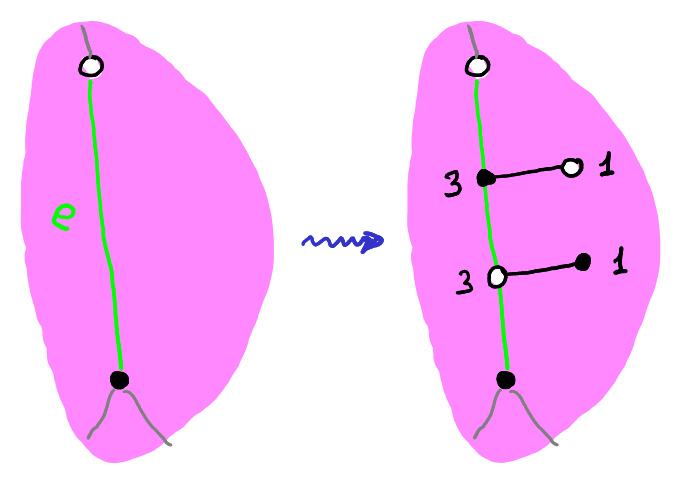
\includegraphics[width=\linewidth]{special-family-5}
\end{center}
\end{manycases}
There are only five families of candidate data satisfying the conditions in the statement.
\begin{enumerate}
\item $\mathcal{D}=\datum{\Sigma_g,6g}{[3,\ldots,3],[3,\ldots,3],[s,6g-s]}$. The realizability of this datum can be deduced by forgetting the augmentation of the data described in step \caseref{3}.
\item $\mathcal{D}=\datum{\Sigma_g,6g+2}{[2,3,\ldots,3],[2,3,\ldots,3],[s,6g+2-s]}$. This datum can be realized by applying step \caseref{4} to the augmented datum
\[
\datum{\Sigma_g,6g}{[3,\ldots,3],[3,\ldots,3],[s,\env{6g-s}]},
\]
which is realizable by step \caseref{3} (assuming $s\le 3g+1$).
\item $\mathcal{D}=\datum{\Sigma_g,6g+3}{[3,\ldots,3],[1,2,3,\ldots,3],[s,6g+3-s]}$. This datum can be realized by applying step \caseref{5} to the augmented datum
\[
\datum{\Sigma_g,6g}{[3,\ldots,3],[3,\ldots,3],[s,\env{6g-s}]},
\]
which is realizable by step \caseref{3} (assuming $s\le 3g+1$).
\item $\mathcal{D}=\datum{\Sigma_g,6g+4}{[1.3,\ldots,3],[1,3,\ldots,3],[s,6g+4-s]}$. This datum can be realized by applying step \caseref{6} to the augmented datum
\[
\datum{\Sigma_g,6g}{[3,\ldots,3],[3,\ldots,3],[s,\env{6g-s}]},
\]
which is realizable by step \caseref{3} (assuming $s\le 3g+2$).
\item $\mathcal{D}=\datum{\Sigma_g,6g+6}{[1,2,3,\ldots,3],[1,2,3,\ldots,3],[s,6g+6-s]}$. This datum can be realized by applying step \caseref{4} twice to the augmented datum
\[
\datum{\Sigma_g,6g}{[3,\ldots,3],[3,\ldots,3],[s,\env{6g-s}]},
\]
which is realizable by step \caseref{3} (assuming $s\le 3g+3$).
\end{enumerate}
The proof is therefore complete.
\end{proof}

\begin{theorem}
Let $\mathcal{D}=\datum{\Sigma_g,d}{\pi_1,\pi_2,[s,d-s]}$ be a proper candidate datum with $g\ge 2$. Then $\mathcal{D}$ is realizable.
\end{theorem}
\begin{proof}
Thanks to \cref{th:exceptional-n3-s1} we can assume that $2\le s\le d-2$. We then proceed by induction on $g\ge 2$.

\begin{manycases}
\case Assume that $d\le 18$. Using Zheng's algorithm, a list of all the proper exceptional candidate data has been computed. It turns out that $\mathcal{D}$ is always realizable.

\case Assume that
\begin{enumerate}
\item there is an element $x\in\pi_1$ such that $x\ge 4$;
\item $2\in\pi_2$.
\end{enumerate}
By applying \cref{move:4-2}, we can reduce the problem to the realizability of the candidate datum
\[
\mathcal{D}'=\datum{\Sigma_{g-1},d-2}{\pi_1\setminus[x]\cup[1,x-3],\pi_2\setminus[2],[s-1,d-s-1]},
\]
which is realizable by \cref{th:exceptional-n3-g1} if $g=2$ (by case \caseref{1} we can assume that $d-2\ge 17$), or by induction if $g\ge 3$.

\case Assume that:
\begin{enumerate}
\item there is an element $x\in\pi_1$ such that $x\ge 4$;
\item there is an element $y\in\pi_2$ such that $y\ge 4$.
\end{enumerate}
We can further assume that $2\not\in\pi_2$ and $2\not\in\pi_2$, otherwise we are done by case \caseref{2}. By applying \cref{move:4-3}, we can reduce the problem to the realizability of the candidate datum
\[
\mathcal{D}'=\datum{\Sigma_{g-1},d-2}{\pi_1\setminus[x]\cup[x-2],\pi_2\setminus[y]\cup[y-2],[s-1,d-s-1]},
\]
which is realizable by \cref{th:exceptional-n3-g1} if $g=2$, or by induction if $g\ge 3$.

\case Assume that:
\begin{enumerate}
\item there is an element $x\in\pi_1$ such that $x\ge 4$;
\item $3\in\pi_2$.
\end{enumerate}
By applying \cref{move:4-3}, we can reduce the problem to the realizability of the candidate datum
\[
\mathcal{D}'=\datum{\Sigma_{g-1},d-2}{\pi_1\setminus[x]\cup[x-2],\pi_2\setminus[3]\cup[1],[s-1,d-s-1]},
\]
which is realizable by \cref{th:exceptional-n3-g1} if $g=2$ (by case \caseref{1} we can assume that $d-2\ge 17$), or by induction if $g\ge 3$.

\case Assume that $3\in\pi_1$. We can further assume that $\max(\pi_1)=3$ and $\max(\pi_2)\le 3$, otherwise the situation is already covered by cases \caseref{2}, \caseref{3} and \caseref{4}. We analyze different sub-cases.

\begin{manycases}[Case \arabic{casei}.\arabic*:]
\case $[1,1]\subs\pi_1$. By \cref{move:113} we have
\[
\mathcal{D}\cmove\datum{\Sigma_{g-1},d}{\pi_1\setminus[3]\cup[1,1,1],\pi_2,[s,d-s]},
\]
which is realizable by \cref{th:exceptional-n3-g1} if $g=2$, or by induction if $g\ge 3$.
\case $[3,3]\subs\pi_1$ and $[2,2]\subs\pi_2$. If $s=2$ or $s=d-2$ then $\mathcal{D}$ is realizable by \cref{move:s2-23-22}. Otherwise, by \cref{move:33-22} we have
\[
\mathcal{D}\cmove\datum{\Sigma_{g-1},d-4}{\pi_1\setminus[3,3]\cup[1,1],\pi_2\setminus[2,2],[s-2,d-s-2]},
\]
which is realizable by \cref{th:exceptional-n3-g1} if $g=2$, or by induction if $g\ge 3$.
\case $[2,2]\not\subs\pi_2$. The Riemann-Hurwitz condition \eqref{eq:rh-n3} immediately implies that $[3,3]\subs\pi_2$. Assume by contradiction that $\mathcal{D}$ is not realizable. Then $[1,1]\not\subs\pi_1$ and $[1,1]\not\subs\pi_2$ (case \caseref{5.1}), and moreover $[2,2]\not\subs\pi_1$ (case \caseref{5.2}). In other words, both $\pi_1$ and $\pi_2$ can be written as $\rho\cup[3,\ldots,3]$, where $\rho\subs[1,2]$ (possibly different for $\pi_1$ and $\pi_2$). As a consequence, by \cref{th:exceptional-n3-special-family}, $\mathcal{D}$ is realizable.
\case $[3,3]\not\subs\pi_1$. From the Riemann-Hurwitz condition \eqref{eq:rh-n3} it follows that $[3,3]\subs\pi_2$, but then $\mathcal{D}$ is realizable by cases \caseref{5.2} and \caseref{5.3}.
\end{manycases}
\end{manycases}

The cases we have analyzed (up to swapping $\pi_1$ and $\pi_2$) cover all the proper candidate data of the form $\datum{\Sigma_g,d}{\pi_1,\pi_2,[s,d-s]}$ with $g\ge 2$. We have showed that every datum is realizable, therefore the proof is complete.
\end{proof}

\end{document}